\documentclass[fleqn, 11pt]{article}

\usepackage{verbatim}
\usepackage{amsmath}
\DeclareMathOperator*{\argmin}{arg\,min}
\usepackage{amssymb}
\usepackage{amsthm}
\usepackage{hyperref}
\usepackage{ulem}
\usepackage{enumitem}
\usepackage[left=0.75in, right=0.75in, bottom=0.75in]{geometry}
\usepackage{graphicx}

\usepackage{import}

\newcommand{\bs}[1]{\boldsymbol{#1}}
\newcommand\norm[1]{\left\lVert#1\right\rVert}

\usepackage{array}
\usepackage{caption}
\usepackage{floatrow}
\usepackage{multirow}

\usepackage{chngcntr}
\counterwithin*{equation}{section}
\counterwithin*{equation}{subsection}

\usepackage{sectsty}
\sectionfont{\centering}

\usepackage[perpage]{footmisc}

\usepackage{fancyhdr}
\pagestyle{fancy}
\fancyhf{}
\lhead{190100036 \& 190100044}
\rhead{CS 754: Assignment 3}
\renewcommand{\footrulewidth}{1.0pt}
\cfoot{Page \thepage}

\setlength{\parindent}{0em}
\renewcommand{\arraystretch}{2}%

\title{Assignment 3: CS 754}
\author{ 
\begin{tabular}{|c|c|}
     \hline
     \textsf{Krushnakant Bhattad} & \textsf{Devansh Jain} \\
     \hline
     \textsf{190100036} & \textsf{190100044}\\
     \hline
\end{tabular}
}
\date{March 23, 2021}

\begin{document}

\maketitle
\tableofcontents
\thispagestyle{empty}
\setcounter{page}{0}

\newpage
\section*{Question 1}
\addcontentsline{toc}{section}{Question 1}
\setcounter{equation}{0}


\subsection*{(a) Restricted Eigenvalues Condition}

We say that a matrix $\bs{X}$ satisfies the restricted eigenvalues condition 
with respect to a constraint set $\mathcal{C}$ 
if there exists a constant $\gamma>0$ such that the following holds 
for all non-zero $  \nu \in \mathcal{C} $:\\

\begin{center}
   $\dfrac{\frac{1}{N} \nu^T \bs{X}^T\bs{X} \nu }{ \norm{\nu}_{\ell_2}^2 } \geq \gamma $
\end{center}

Equivalently:

\begin{center}
   $\dfrac{\frac{1}{N} \norm{\bs{X} \nu}_{\ell_2}^2 }{ \norm{\nu}_{\ell_2}^2 } \geq \gamma $
\end{center}

 
~\\If we have the above condition, that the quantity on the LHS is bounded away from zero, 
then we know we have enough curvature so that a small loss difference implies a small error.



\subsection*{(b) Starting from equation 11.20 $\ldots$}

We know that $\hat{\beta}$ is the minimizer of 

\begin{center}
    $K(\beta)= (1/2N) \norm{\bs{y-X \beta}}_{\ell_2}^2 + \lambda_N \norm{\bs{\beta}}_{\ell_1} $, 
\end{center}

that is we know that:

\begin{center}
    
$(1/2N) \norm{\bs{y-X \hat{\beta}}}_{\ell_2}^2 + \lambda_N \norm{\hat{\bs{\beta}}}_{\ell_1}  
\leq  (1/2N) \norm{\bs{y-X \beta^*}}_{\ell_2}^2 + \lambda_N \norm{\bs{\beta}^*}_{\ell_1} $

\end{center}


Due to this it follows from definition of $G$ that $G(\hat{\nu}) \leq G(0)$

\newpage
\includegraphics[scale=0.27]{CS754_HW3_Q1c.jpg}

\newpage
\includegraphics[scale=0.37]{CS754_HW3_Q1d.jpg}

\newpage
\includegraphics[scale=0.27]{CS754_HW3_Q1e1.jpg}


\includegraphics[scale=0.27]{CS754_HW3_Q1e2.jpg}

\newpage
\includegraphics[scale=0.27]{CS754_HW3_Q1f.jpg}

\newpage
\includegraphics[scale=0.25]{CS754_HW3_Q1g.jpg}

\newpage

\subsection*{(h) Why is the cone constraint required? }

It is clear that the following least-squares objective function is always convex.

\begin{center}
    $f_N(\beta) = \dfrac{1}{2N} \norm{\bs{y - X \beta}}_2^2$
\end{center}


What we desire is that whenever the difference in function values $\Delta f_N = | f_N(\beta_1) - f_N(\beta_2) |  $
converges \\ to zero, the $\ell_2$-norm
of the parameter vector difference $\Delta \beta = \norm{ \beta_1 - \beta_2 }_2    $ also converges to zero. 

\smallskip

This notion is a strengthening of ordinary
convexity, hence called strong convexity.

\medskip

$f_N(\beta)$ is also strongly convex whenever the eigenvalues of the 
$p \times p$ positive semi-definite matrix $\bs{X^TX}$ 
are uniformly bounded away from zero.

\smallskip 

Simple linear algebra shows that if $N < p$, the matrix $\bs{X^TX}$ (which always has 
rank at most $\min\{N, p\}$) is always rank-deficient and thus not strongly convex.

\medskip

For this reason, we need to relax our notion of strong convexity. 
Well we're anyway concerned about about a particular set 
that only contains some specific sparse vectors; hence we will see the 
condition constrained to that set only. 

\smallskip

In the current condition, we suppose that the parameter vector $\beta^*$ is sparse - say supported on some 
subset $S=S(\beta^*)$. 

\smallskip

The restricted eigenvalues condition considers the corresponding
specific constraint set $\mathcal{C}$, in which we can achieve restricted strong convexity. 
These notions are related because for this objective function, the hessian matrix 
$\nabla^2 f(\beta) $   is proportional to  $ \bs{X^TX}$  

\medskip

The LASSO error is defined as $\hat{\nu} = \hat{\beta}- \beta^*$. 

\smallskip

Let $\hat{\nu}_S$ denote the subvector indexed by elements of S, and 
let $\hat{\nu}_{S^c}$ defined in an analogous manner.

\smallskip

As we proved in the lemma 11.1, it turns out (in those particular conditions, where it is called regularized form)
that the lasso error satisfies a cone constraint of the form
$\norm{\hat{\nu}_{S^c}}_1 \leq 3   \norm{\hat{\nu}_S}_1$ 

\medskip

For the constrained lasso with ball radius $R = \norm{\beta^*}_1$, 
it can be proved that $\norm{\hat{\nu}_{S^c}}_1 \leq  \norm{\hat{\nu}_S}_1$  

\medskip

A general cone constraint is $\norm{\hat{\nu}_{S^c}}_1 \leq  \alpha  \norm{\hat{\nu}_S}_1$  
for some constant $\alpha \geq 1$.

\medskip

Thus, in
either its constrained or regularized form, the lasso error is restricted to a set
of the form 


\begin{center}
    
$\mathcal{C}(S ; \alpha) : = \{ \nu \in \mathbb{R}^p \text{ such that } 
\norm{\hat{\nu}_{S^{c}}}_1 \leq \alpha \norm{\hat{\nu}_{S}}_1 \}$
for some parameter $\alpha \geq 1$. 

\end{center}

Thus by the cone constraint we achieve strong convexity in the region of the lasso error,
which thus helps us achieve our goal, that is,
whenever the difference in function values $\Delta f_N = | f_N(\beta_1) - f_N(\beta_2) |  $
converges to zero, the $\ell_2$-norm
of the parameter vector difference 
$\Delta \beta = \norm{ \beta_1 - \beta_2 }_2    $ also converges to zero. 

\bigskip


\newpage
\subsection*{(i)  This theorem Vs Theorem 3 that we did in class.}
\begin{enumerate}
    \item There was a restriction on the value of $\delta_{2S}$ ($< \sqrt{2} - 1$) in Theorem 3, here, there is no restriction on $\gamma$ (except $> 0$) in this Theorem.
    \item As described on Pg. 296, ``the rate (11.15)—including the logarithmic factor—is known to be minimax optimal, meaning that it cannot be substantially improved upon by any estimator.".
    \item On Pg. 302, Theorem 11.3 states the uniqueness of the optimal solution $\hat{\beta}$, no false inclusions and exclusions of indices; and hence is variable selection consistent.
    \item On applying Theorem 3 with error modelled as zero-mean Gaussian with standard deviation $\sigma$, we choose $\epsilon$ as $9m\sigma^2$ (whp), which gives the error bound proportional to $\sigma^2$.\\
    In this example, we showed that taking $\lambda_N$ proportional to $\sigma$ is also a valid choice, with high probability; which provides a tighter bound than Theorem 3.
    \item In this theorem, we have restricted $\beta*$ to be a k-sparse vector, i.e. sparse in basis $\mathbf{X}$. \\
    Theorem 3 has the advantage that it gives error bounds for compressible signals as well.
\end{enumerate}

\bigskip


\subsection*{(j) What is the common thread between the bounds on the `Dantzig selector' and the LASSO?}

$\sigma_k(x)$ is defined on Pg. 12 as the error incurred by approximating a signal $x$ by some $\hat{x} \in \Sigma_k$: $$\sigma_k (x)_p = \min_{\hat{x} \in \Sigma_k} ||x - \hat{x}||_p.$$
If $x \in \Sigma_k$, then clearly $\sigma_k (x)_p = 0$ for any $p$.\\

\begin{enumerate}
    \item The theorem on LASSO error bound (Theorem 11.1) considering the signal $\beta*$ to be k-sparse. \\
        The error bound obtained is proportional to $\sqrt{k}$. \\
        If we apply the same condition on the signal $x$ while using `Dantzig selector' and using bounds mentioned (Theorem 1.10), the first term of the error bound would reduce to zero, thus making the error bound proportional to $\sqrt{k}$, same as above.
    \item The bounds in LASSO estimation is proportional to the regularization parameter $\lambda_N \ge 2 ||\mathbf{X}^T \mathbf{w} ||_{\infty}/N$. \\
        Upon applying similar condition, the bounds of `Dantzig selector' are proportional to $\lambda \ge || A^T e ||_{\infty}$.
\end{enumerate}


\bigskip

\newpage
\subsection*{(k) What is the advantage of the square-root LASSO over the LASSO?}

\subsubsection*{The LASSO:}

The LASSO solves the following, where $ \bs{y} \in \mathbb{R}^n$, $ \bs{X} \in \mathbb{R}^{n \times p} $ :

\begin{center}
    
$\hat{\beta} \in \displaystyle 
\argmin_{\beta \in \mathbb{R}^p} \dfrac{\norm{\bs{y-X \beta}}_{\ell_2}^2}{n}
+ \dfrac{\lambda}{n} \norm{\beta}_{\ell_1} \hspace{20pt}\ldots(1) $   

\end{center}

with a suitable penalty level: $\lambda = c \cdot ( 2 \sigma \sqrt{n} \Phi^{-1/2}(1-\alpha / 2p) ) $
where: 
$c>1$ is some constant, $\sigma$ is the standard deviation of noise, $n$ is the number of observation samples, 
and $\Phi$ is the Gaussian probability distribution function.

\subsubsection*{The square root LASSO:}

The square root LASSO solves the following: 

\begin{center}
    
$\hat{\beta} \in \displaystyle 
\argmin_{\beta \in \mathbb{R}^p} \sqrt{\dfrac{\norm{\bs{y-X \beta}}_{\ell_2}^2}{n}}
+ \dfrac{\lambda}{n} \norm{\beta}_{\ell_1}   \hspace{20pt}\ldots(1)   $

\end{center}

where the suitable penalty level is: $\lambda = c \cdot ( \sqrt{n} \Phi^{-1/2}(1-\alpha / 2p) ) $

All the terms have same meanings as above.

\subsubsection*{Advantages of the square root LASSO: }


We observe that, in (2), the penalty level is independent of $\sigma$, the noise variance, 
which is contrasting with what we observed in (1). This observation is used in point 3 below.

\medskip 

Here are some advantages of the square root LASSO:
\begin{enumerate}
    \item Despite taking the square-root of the least squares criterion function, the square root LASSO retains global convexity, making the estimator as computationally attractive as LASSO
    \item The square-root LASSO can be formulated as a solution to a conic programming problem.
    \item The original LASSO construction relies on knowing the standard deviation $\sigma$ of the noise. Estimation of $\sigma$  is nontrivial when p is large, particularly when $ p \gg n $, and remains an outstanding practical and theoretical problem. The square root LASSO eliminates the need to know or to pre-estimate $\sigma$. 
    \item By using moderate deviation theory, we can do away with the assumption that noise follows the normal distribution under certain conditions.
\end{enumerate}

Thus while keeping many of the advantages of LASSO intact, the square root LASSO 
adds more features to it.

\newpage
\section*{Question 2}
\addcontentsline{toc}{section}{Question 2}
\setcounter{equation}{0}

\subsection*{Instructions for running the code:}
\begin{itemize}[noitemsep]
    \item After extracting submitted file, look for a directory named \texttt{q2}, and \texttt{cd} (change directory) to it.
    \item Run the files \texttt{q2a.m}, \texttt{q2b.m}, \texttt{q2c.m} and \texttt{q2d.m}. The results can be found in \texttt{./results/}.
\end{itemize}

\subsection*{Package l1\_ls\_matlab}
Passing \texttt{A} and \texttt{At} as objects
\begin{verbatim}
Usage: [x,status]=l1_ls(A,At,m,n,y,lambda,rel_tol);
\end{verbatim}

\subsection*{Common Steps}
\begin{enumerate}[noitemsep]
    \item Reading the slice(s)
    \item Padding the slice(s) to form square slice(s)
    \item Angles of Projection\footnote{Even though the question mentions to randomly generate projection angles, best results are found when the projection angles are uniformly spaced. Confirmed with Professor.}
    \item Creating Tomographic Projections
    \item Creating objects of Forward matrix (omitted in (a))
    \item Reconstruction using
    \begin{enumerate}[noitemsep]
        \item Filtered Back-projection with Ram-Lak filter
        \item Compressed Sensing
        \item 2 slice Coupled Compressed Sensing
        \item 3 slice Coupled Compressed Sensing
    \end{enumerate}
    \item Result
\end{enumerate}

\subsection*{(b) Compressed Sensing}
\subsubsection*{Minimization function}
\begin{equation*}
    \begin{aligned}
        & \argmin_\beta \ \lVert \mathbf{y} - \mathbf{R}\mathbf{U}\mathbf{\beta} \rVert^2 + \lambda \lVert \mathbf{\beta} \rVert_1
    \end{aligned}
\end{equation*}

\subsubsection*{Class RU}
Class \texttt{RU} present under folder \texttt{@RU}.\\
\texttt{@RU/RU.m} contains class constructor.\\
\texttt{@RU/ctranspose.m} contains overloaded transpose operator (').\\
\texttt{@RU/mtimes.m} contains overloaded product operator (*).\\


\subsection*{(c) 2 slice Coupled Compressed Sensing}
\subsubsection*{Minimization function}
\begin{equation*}
    \begin{aligned}
        & \argmin_{\beta_1, \beta_2} \ \lVert y_1 - R_1 U \beta_1 \rVert^2 + \lVert y_2 - R_2 U \beta_2  \rVert^2 + \lambda \lVert \beta_1  \rVert_1 + \lambda \lVert \beta_1 - \beta_2 \rVert_1 \\
        &= \argmin_{\beta_1, \Delta\beta} \ \lVert y_1 - R_1 U \beta_1 \rVert^2 + \lVert y_2 - R_2 U (\beta_1 + \Delta\beta) \rVert^2 + \lambda \lVert \beta_1 \rVert_1 + \lambda \lVert \Delta\beta \rVert_1 \\
        &= \argmin_{\beta_1, \Delta\beta} \ \left\lVert \begin{pmatrix} y_1 \\ y_2 \end{pmatrix} - \begin{pmatrix} R_1 U & 0 \\ R_2 U & R_2 U \end{pmatrix} \begin{pmatrix} \beta_1 \\ \Delta\beta \end{pmatrix} \right\rVert^2 + \lambda \left\lVert \begin{pmatrix} \beta_1 \\ \Delta\beta \end{pmatrix} \right\rVert_1 \\
        & \text{ where, } \beta_2 = \beta_1 + \Delta\beta
    \end{aligned}
\end{equation*}

\subsubsection*{Class CCS2}
Class \texttt{CCS2} present under folder \texttt{@CCS2}.\\
\texttt{@CCS2/CCS2.m} contains class constructor.\\
\texttt{@CCS2/ctranspose.m} contains overloaded transpose operator (').\\
\texttt{@CCS2/mtimes.m} contains overloaded product operator (*).\\


\subsection*{(d) 3 slice Coupled Compressed Sensing}
\subsubsection*{Minimization function}
\begin{equation*}
    \begin{aligned}
        & \argmin_{\beta_1, \beta_2, \beta3} \ \lVert y_1 - R_1 U \beta_1 \rVert^2 + \lVert y_2 - R_2 U \beta_2 \rVert^2 + \lVert y_3 - R_3 U \beta_3 \rVert^2 + \lambda \lVert \beta_2  \rVert_1 + \lambda \lVert \beta_2 - \beta_1 \rVert_1 + \lambda \lVert \beta_2 - \beta_3 \rVert_1 \\
        &= \argmin_{\beta_2, \Delta\beta_1, \Delta\beta_2} \ \lVert y_1 - R_1 U (\beta_2 + \Delta\beta_1) \rVert^2 + \lVert y_2 - R_2 U \beta_2 \rVert^2 + \lVert y_3 - R_3 U (\beta_2 + \Delta\beta_2) \rVert^2 + \lambda \lVert \beta_2 \rVert_1 + \lambda \lVert \Delta\beta_1 \rVert_1 + \lambda \lVert \Delta\beta_2 \rVert_1 \\
        &= \argmin_{\beta_2, \Delta\beta_1, \Delta\beta_2} \ \left\lVert \begin{pmatrix} y_1 \\ y_2 \\ y_3 \end{pmatrix} - \begin{pmatrix} R_1 U & R_1 U & 0 \\ R_2 U & 0 & 0 \\ R_3 U & 0 & R_3 U \end{pmatrix} \begin{pmatrix} \beta_2 \\ \Delta\beta_1 \\ \Delta\beta_2 \end{pmatrix} \right\rVert^2 + \lambda \left\lVert \begin{pmatrix} \beta_2 \\ \Delta\beta_1 \\ \Delta\beta_2 \end{pmatrix} \right\rVert_1
         & \text{ where, } \beta_1 = \beta_2 + \Delta\beta_1 \text{ and } \beta_3 = \beta_2 + \Delta\beta_2
   \end{aligned}
\end{equation*}

\subsubsection*{Class CCS3}
Class \texttt{CCS3} present under folder \texttt{@CCS3}.\\
\texttt{@CCS3/CCS3.m} contains class constructor.\\
\texttt{@CCS3/ctranspose.m} contains overloaded transpose operator (').\\
\texttt{@CCS3/mtimes.m} contains overloaded product operator (*).\\


\subsection*{Results}
\begin{figure}[H]
    \centering
    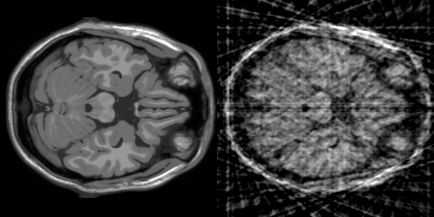
\includegraphics[scale=0.6]{q2a.png}
    \caption{Original (\texttt{slice50.png}) Vs Reconstruction from Tomographic Projections (18 angles) using Filtered Back-projection}
\end{figure}

\begin{figure}[H]
    \centering
    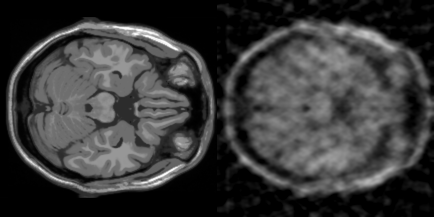
\includegraphics[scale=0.6]{q2b_100.png}
    \caption{Original (\texttt{slice50.png}) Vs Reconstruction from Tomographic Projections (18 angles) using Compressed Sensing with $\lambda = 100$}
\end{figure}
\begin{figure}[H]
    \centering
    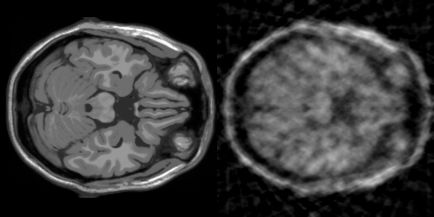
\includegraphics[scale=0.6]{q2b_10.png}
    \caption{Original (\texttt{slice50.png}) Vs Reconstruction from Tomographic Projections (18 angles) using Compressed Sensing with $\lambda = 10$}
\end{figure}
\begin{figure}[H]
    \centering
    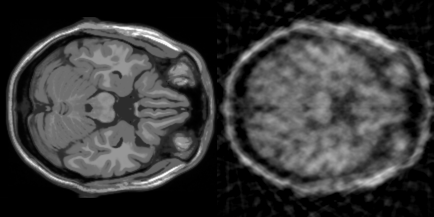
\includegraphics[scale=0.6]{q2b_1.png}
    \caption{Original (\texttt{slice50.png}) Vs Reconstruction from Tomographic Projections (18 angles) using Compressed Sensing with $\lambda = 1$}
\end{figure}
\begin{figure}[H]
    \centering
    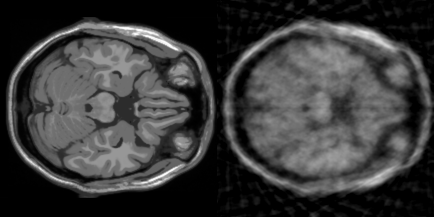
\includegraphics[scale=0.6]{q2b_0.1.png}
    \caption{Original (\texttt{slice50.png}) Vs Reconstruction from Tomographic Projections (18 angles) using Compressed Sensing with $\lambda = 0.1$}
\end{figure}
\begin{figure}[H]
    \centering
    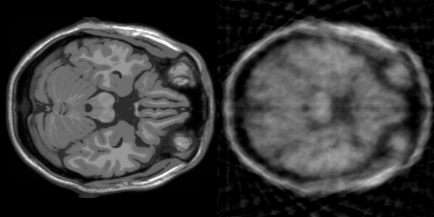
\includegraphics[scale=0.6]{q2b_0.01.png}
    \caption{Original (\texttt{slice50.png}) Vs Reconstruction from Tomographic Projections (18 angles) using Compressed Sensing with $\lambda = 0.01$}
\end{figure}

\begin{figure}[H]
    \centering
    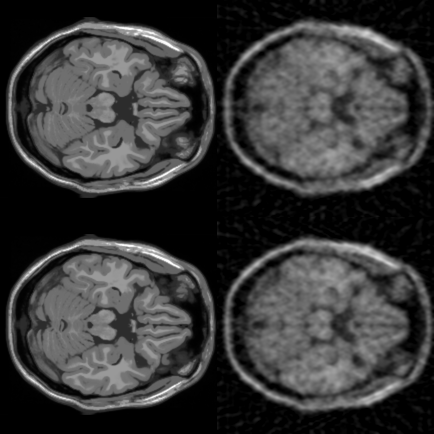
\includegraphics[scale=0.6]{q2c_100.png}
    \caption{Original (\texttt{slice51.png}, \texttt{slice52.png}) Vs Reconstruction from Tomographic Projections (18 angles) using 2 slice Coupled Compressed Sensing with $\lambda = 100$}
\end{figure}
\begin{figure}[H]
    \centering
    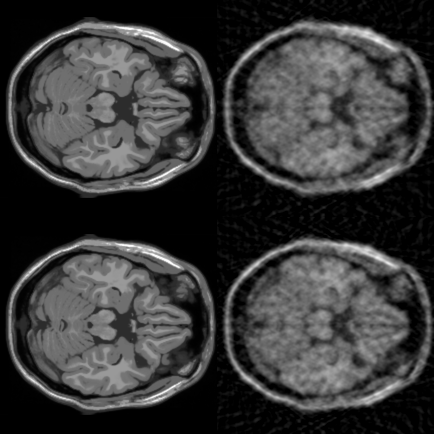
\includegraphics[scale=0.6]{q2c_10.png}
    \caption{Original (\texttt{slice51.png}, \texttt{slice52.png}) Vs Reconstruction from Tomographic Projections (18 angles) using 2 slice Coupled Compressed Sensing with $\lambda = 10$}
\end{figure}
\begin{figure}[H]
    \centering
    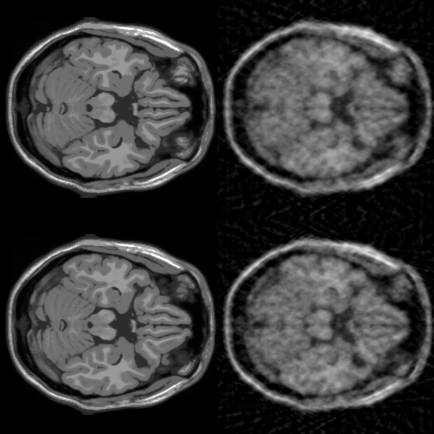
\includegraphics[scale=0.6]{q2c_1.png}
    \caption{Original (\texttt{slice51.png}, \texttt{slice52.png}) Vs Reconstruction from Tomographic Projections (18 angles) using 2 slice Coupled Compressed Sensing with $\lambda = 1$}
\end{figure}
\begin{figure}[H]
    \centering
    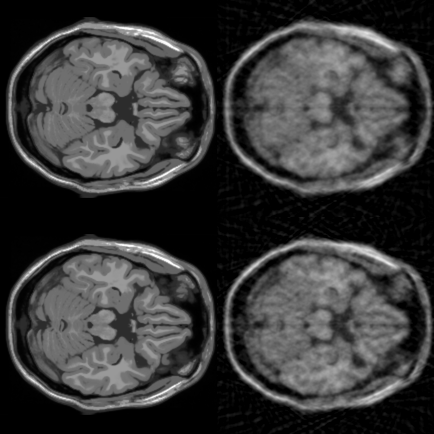
\includegraphics[scale=0.6]{q2c_0.1.png}
    \caption{Original (\texttt{slice51.png}, \texttt{slice52.png}) Vs Reconstruction from Tomographic Projections (18 angles) using 2 slice Coupled Compressed Sensing with $\lambda = 0.1$}
\end{figure}

\begin{figure}[H]
    \centering
    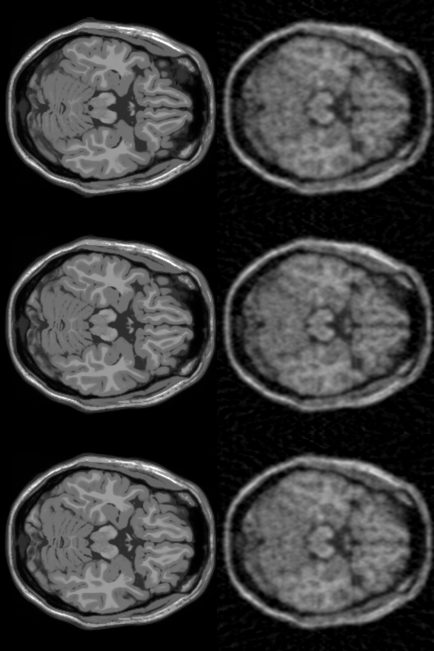
\includegraphics[scale=0.8]{q2d_100.png}
    \caption{Original (\texttt{slice53.png}, \texttt{slice54.png}, \texttt{slice55.png}) Vs Reconstruction from Tomographic Projections (18 angles) using 3 slice Coupled Compressed Sensing with $\lambda = 100$}
\end{figure}
\begin{figure}[H]
    \centering
    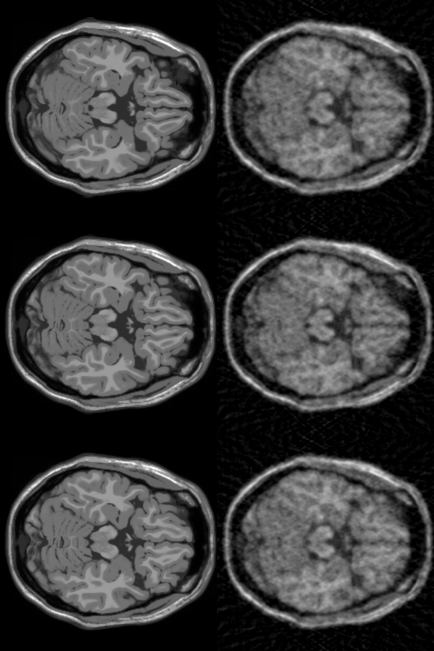
\includegraphics[scale=0.8]{q2d_10.png}
    \caption{Original (\texttt{slice53.png}, \texttt{slice54.png}, \texttt{slice55.png}) Vs Reconstruction from Tomographic Projections (18 angles) using 3 slice Coupled Compressed Sensing with $\lambda = 10$}
\end{figure}
\begin{figure}[H]
    \centering
    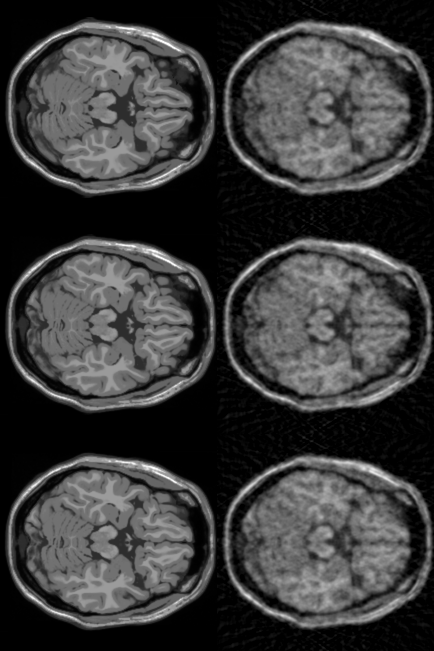
\includegraphics[scale=0.8]{q2d_1.png}
    \caption{Original (\texttt{slice53.png}, \texttt{slice54.png}, \texttt{slice55.png}) Vs Reconstruction from Tomographic Projections (18 angles) using 3 slice Coupled Compressed Sensing with $\lambda = 1$}
\end{figure}


\newpage
\section*{Question 3}
\addcontentsline{toc}{section}{Question 3}
\setcounter{equation}{0}

\subsection*{(a) Shifting:}

$LHS 
= R(g(x-x_0,y-y_0))(\rho, \theta)
= \displaystyle \int_{-\infty }^{\infty} \int_{-\infty }^{\infty}  g(x-x_0,y-y_0) \delta (\rho - x \cos \theta - y \sin \theta) dx dy
$

 \smallskip 

Now we'll do a change of variables. Let $x'=x-x_0$ and $y'=y-y_0$.

 \medskip 

Thus we get,

 \smallskip 

$LHS 
= \displaystyle \int_{-\infty }^{\infty} \int_{-\infty }^{\infty}  g(x',y') \delta (\rho - x_0 \cos \theta - y_0 \sin \theta - x' \cos \theta - y' \sin \theta) dx dy 
$

 \smallskip 

$
= \displaystyle \int_{-\infty }^{\infty} \int_{-\infty }^{\infty}  g(x',y') \delta ( (\rho - x_0 \cos \theta - y_0 \sin \theta) - x' \cos \theta - y' \sin \theta) dx' dy'
$

 \medskip 

If we observe carefully, this is precisely the expression for the radon transform of $g(x,y)$ 
at an angle $\theta$, \\ with offset  
$\rho' = \rho - x_0 \cos \theta - y_0 \sin \theta$ 

 \medskip 

Thus, 

 \smallskip 

$
LHS
=R(g(x-x_0,y-y_0))(\rho, \theta)
= R(g(x,y))(\rho - x_0 \cos \theta - y_0 \sin \theta, \theta) 
=RHS
$

and we're done.

~\\

\hrulefill 


\subsection*{(b) Rotation:}

Using change of variables to polar co-ordinates, the 2D radon transform can be written as: 

\smallskip

$R (f(r, \psi)) (\rho, \theta) 
= \displaystyle \int_{-\pi}^{\pi} \int_{0}^{\infty}  f(r, \psi) \delta (\rho - r \cos \psi \cos \theta - r \sin \psi \sin \theta) r dr d \psi 
$

\medskip

That is, 
$ R (f(r, \psi)) (\rho, \theta) 
= \displaystyle \int_{-\pi }^{\pi} \int_{0}^{\infty}  f(r, \psi) \delta (\rho - r \cos (\psi - \theta) ) r dr d \psi 
$

\medskip

Now let's get to proving. 

\smallskip

$ R (g(r, \psi - \psi_0)) (\rho, \theta)  
= \displaystyle \int_{-\pi }^{\pi} \int_{0}^{\infty}  g(r, \psi - \psi_0) \delta (\rho - r \cos (\psi - \theta) ) r dr d \psi 
$

\medskip

Substitute $\psi' = \psi - \psi_0$. 

\smallskip

$ R (g(r, \psi - \psi_0)) (\rho, \theta)  
= \displaystyle \int_{-\pi - \psi_0 }^{\pi - \psi_0 } \int_{0}^{\infty}  g(r, \psi') \delta (\rho - r \cos (\psi' + \psi_0 - \theta) ) r dr d \psi' 
$

\medskip

Noting that for functions with period $2 \pi$, as is the case here,
$ \displaystyle \int_{-\pi - \psi_0 }^{\pi - \psi_0 } f(\theta) d \theta =  
\displaystyle \int_{-\pi  }^{\pi } f(\theta) d \theta 
$  

\medskip

$ R (g(r, \psi - \psi_0)) (\rho, \theta)  
= \displaystyle \int_{-\pi}^{\pi} \int_{0}^{\infty}  g(r, \psi') \delta (\rho - r \cos (\psi' - ( \theta- \psi_0)) r dr d \psi' 
$

\medskip

which is precisely the required radon transform:

\medskip

$ R (g(r, \psi - \psi_0)) (\rho, \theta)  
= R (g(r, \psi)) (\rho, \theta - \psi_0 )
$




\newpage 

\subsection*{(c) Convolution:}


$(f * k) (x,y) = \displaystyle \int_{-\infty }^{\infty} \int_{-\infty }^{\infty}  f(x_1,y_1) k(x-x_1, y-y_1) dx_1 dy_1$

\bigskip

The radon transform of this is: 

\medskip 

$R((f * k) (x,y)) (\rho, \theta) 
$

\smallskip

$
=   \displaystyle \int_{-\infty }^{\infty} \int_{-\infty }^{\infty} \int_{-\infty }^{\infty} \int_{-\infty }^{\infty}  f(x_1,y_1) k(x-x_1, y-y_1) \delta (\rho - x \cos \theta - y \sin \theta)  
dx_1 dy_1 dx dy  $

\bigskip 

Assuming the functions are ``nice", and using properties of multiple integrals we can change 
the order of integration as follows:

\medskip 

$R((f * k) (x,y)) (\rho, \theta) 
$


\smallskip

$
=   \displaystyle \int_{-\infty }^{\infty} \int_{-\infty }^{\infty} f(x_1,y_1) \left[ \int_{-\infty }^{\infty} \int_{-\infty }^{\infty}   k(x-x_1, y-y_1) \delta (\rho - x \cos \theta - y \sin \theta)  dx dy \right]
dx_1 dy_1   $

\bigskip

By the shifting property proved in $(a)$, we can write the integral in the square brackets  as:

\medskip 

$R((f * k) (x,y)) (\rho, \theta) 
$


\smallskip

$
=   \displaystyle \int_{-\infty }^{\infty} \int_{-\infty }^{\infty} f(x_1,y_1) \left[ R(k(x,y))(\rho - x_1 \cos \theta - y_1 \sin \theta, \theta) \right]
dx_1 dy_1   $


~\\

Since $ \displaystyle \int_{-\infty }^{\infty} f(x) \delta(x-x') dx= f(x')$, 

we have 


$
R(k(x,y))(\rho - x_1 \cos \theta - y_1 \sin \theta, \theta)
=  \displaystyle \int_{-\infty }^{\infty} R(k(x,y))(\rho - \rho_1, \theta) \delta ( \rho_1 - x_1 \cos \theta - y_1 \sin \theta  ) d \rho_1
$

Thus we can write, 


\medskip 

$R((f * k) (x,y)) (\rho, \theta) 
$


\smallskip

$
=   \displaystyle \int_{-\infty }^{\infty} \int_{-\infty }^{\infty} \int_{-\infty }^{\infty} f(x_1,y_1)  
R(k(x,y))(\rho - \rho_1, \theta) \delta ( \rho_1 - x_1 \cos \theta - y_1 \sin \theta  )
dx_1 dy_1 d \rho_1   $


\bigskip


Regrouping the terms, we have: 


\medskip 

$R((f * k) (x,y)) (\rho, \theta) 
$


\smallskip

$
=   \displaystyle \int_{-\infty }^{\infty} R(k(x,y))(\rho - \rho_1, \theta) \left[ \int_{-\infty }^{\infty} \int_{-\infty }^{\infty} f(x_1,y_1)  
 \delta ( \rho_1 - x_1 \cos \theta - y_1 \sin \theta  )
dx_1 dy_1 \right] d \rho_1   $


\bigskip

Again, the terms in the square bracket allow us to write: 


\medskip 

$R((f * k) (x,y)) (\rho, \theta) 
$


\smallskip

$
=   \displaystyle \int_{-\infty }^{\infty} R(k(x,y))(\rho - \rho_1, \theta) 
R(f(x,y)) (\rho_1, \theta ) 
d \rho_1   $


\bigskip

which is in fact the desired convolution, allowing us to write,


\medskip 

$R((f * k) (x,y)) (\rho, \theta) 
$


\smallskip

$
= R(f(x,y))  (\rho, \theta)  * R(k(x,y))  (\rho, \theta) 
$


\bigskip



\newpage
\section*{Question 4}
\addcontentsline{toc}{section}{Question 4}
\setcounter{equation}{0}

\textbf{Claim. } Let $\bs{A}$ be the sensing matrix, 
such that every column of it is unit normalised.

If $\bs{A}$ has s-order restricted isometry constant $\delta_s$ 
and mutual coherence $\mu$, 
$\delta_s \leq (s-1) \mu $ 


\hrulefill 

\medskip

\textbf{Proof:}
\smallskip

Let $S$ be a subset of columns of $\bs{A}$ with $|S|=s$. 

\medskip 

Then, $\bs{A_S^TA_S}$ is a symmetric positive semi definite matrix. 

\medskip 

Let $\lambda_{max}$ and $\lambda_{min}$ be the largest and smallest eigenvalues of $\bs{A_S^TA_S}$ . 

We have, $\lambda_{max} \geq   \lambda_{min} \geq 0$


Suppose $\bs{x}$ be a $s-$sparse vector with the non-zero values in subset corresponding to $S$. 

Then,
\begin{align*}
    \norm{\bs{Ax}}^2 &= \norm{\bs{A_Sx}_S}^2  \\
&= (\bs{A_Sx}_S)^T \bs{A_Sx}_S \\
&= \bs{x}_S^T  \bs{A}_S^T \bs{A_Sx}_S     \\
&= (\bs{A_S^TA_Sx_S})^T \bs{x_S} \\
&=  (\lambda \bs{x_S})^T \bs{x_S}  \hspace{40pt} 
 \ldots \hspace{5pt} \lambda \text{ is some eigenvalue of } \bs{A_S^TA_S}  \\
&= \lambda (\bs{x_S}^T \bs{x_S}) \\
&\leq \lambda_{max} \bs{\norm{x_S}}^2\\
&= \lambda_{max} \bs{\norm{x}}^2
\end{align*}
Similarly,
$\norm{\bs{Ax}} ^2 = \norm{\bs{A_Sx}_S}  ^2 \geq \lambda_{min} \bs{\norm{x}}^2 $

\medskip

Thus, $\lambda_{min} \bs{\norm{x}}^2 \leq \bs{\norm{Ax}}^2 \leq \lambda_{max} \bs{\norm{x}}^2$

\medskip 
Thus we get $\delta_s = \max \{ 1 - \lambda_{min} , \lambda_{max} -1 \}$ . 

\medskip 


\medskip 
Suppose $ \lambda  $ be some eigenvalue of $\bs{A_S^TA_S}$ . 

\medskip 

Gershgorin’s Disk Theorem says that: 

For an eigenvalue $\lambda$ of a square matrix $\bs{B}$ of $n \times n$, there is an index $j \in \{ 1,2,\cdots,n \}$

such that $| \lambda - B_{jj} | \leq \displaystyle \sum_{i=0, i \neq j}^{i=n} |B_{ji} |$

\medskip 

In our case (where we consider $B=\bs{A_S^TA_S}$); due to unit normalisation, we have $(\bs{A_S^TA_S})_{jj}=1$ and  

by definition of mutual coherence, we can also write the following: 

$\displaystyle \sum_{i=0, i \neq j}^{i=s} |(\bs{A_S^TA_S})_{ji} | 
= \sum_{i=0, i \neq j}^{i=s} |((\bs{A_S})_j)^T (\bs{A_S})_{i} |  
\leq \sum_{i=0, i \neq j}^{i=s} \mu(\bs{A}) 
= (s-1) \mu(\bs{A})   $

\medskip 

Therefore we have 

$|\lambda-1|  \leq  (s-1) \mu(\bs{A})  $

\medskip 

Which implies $\lambda_{max} -1  \leq  (s-1) \mu(\bs{A})  $ and $1-\lambda_{min}  \leq  (s-1) \mu(\bs{A})  $ 

\medskip 

Thus finally,
$\delta_s \leq (s-1) \mu $ 



\newpage
\section*{Question 5}
\setcounter{equation}{0}
\addcontentsline{toc}{section}{Question 5}

\textbf{Title} : X‐ray computed tomography for quality inspection of agricultural products: A review \\
\textbf{Venue} : Food Science \& Nutrition - Wiley Online Library \\
\textbf{First published} : 23rd August 2019 \\
\textbf{Link} : \url{https://onlinelibrary.wiley.com/doi/full/10.1002/fsn3.1179}

\subsection*{Mathematical Problem}
X‐ray CT technology is used to obtain two‐dimensional slice images and three‐dimensional tomographic images of samples. The review provides an overview of the working principle of X‐ray CT technology, image processing, and analysis. \\

It models the tomographic projections based on the attenuation intensity as indicated by the \textbf{Beer–Lambert law} (Curry, Dowdey, \& Murry, 1990; Wu, Yang, \& Zhou, 2008; Ying \& Han, 2005).
$$I = I_0 e^{-\mu_n l}$$
where $I$ is the intensity of X‐ray exiting through a sample in eV,\\
$I_0$ is the intensity of X‐ray in eV,\\
$\mu_n$ is the linear attenuation coefficient of a sample on the wavelength in eV/mm, and\\
$l$ is the path length through a sample in mm. \\

The calculation formula of CT number is as follows:
$$ \text{CT Number} = \frac{\mu - \mu_w}{\mu} \times 1000 $$
where $\mu$ is the linear attenuation coefficient of a sample, and\\
$\mu_w$ is the linear attenuation coefficient of water (approximately 0.195).\\
The measurement range of CT number is from –1,000 Hu to + 4,000 Hu. Besides, CT number for air is –1,000 Hu and the number for water is 0 Hu (Ogawa, 1998).

\subsection*{Image Processing and Analysis}
\textbf{Procedure:}
\begin{enumerate}[noitemsep]
    \item 2D slice images are generated to reconstruct the 3D model
    \item Gaussian or median filter is used to reduce noise with 3D raw gray‐level images
    \item The \textbf{threshold segmentation} is used to segment the image based on the gray value histogram of different regions. More on this below.
    \item The final step is the qualitative and quantitative analysis on CT data of region of interests (ROIs).
\end{enumerate}

\begin{figure}[H]
    \centering
    \includegraphics[scale=0.5]{Q5.jpg}
\end{figure}

\newpage 

\subsection*{Optimization Constructs}

In the process, we used optimization in two different steps: 

\medskip

\textbf{3D - reconstruction:}

\smallskip

In the image processing part, we reconstruct the 3D model using various 2D slice images. This can be \\ performed via
various methods like using SURF(Speeded-Up Robust Features), or, say SIFT (Scale-Invariant Feature Transform) 
for feature detection steps: detection, description and matching, which can then be used with methods like 
SSD (Sum of Squared Differences) matching algorithm using image segmentation with aim to obtain 
accurate 3D models. 

These methods involve optimization of parameters like matching cost($D(p)$):

$$D(p)=\exp (-SSD(p))$$

where $SSD(p)$ is the SSD score in a square neighborhood searching window.

We are omitting exact details of this optimization construct; as this is just a tool for accomplishing 
one particular step; however we mentioned this as the question asked for methods of optimization. 

\medskip

\textbf{Threshold segmentation}

\smallskip

In digital image processing, thresholding is a method of
segmenting images. From a grayscale image,
thresholding is used to create binary images.

\smallskip

Automatic thresholding is a great way to extract 
useful information encoded into pixels.

\smallskip

The \textbf{optimization} done for this purpose is to minimize
background noise. 

\smallskip

This is accomplished by utilizing a feedback loop to optimize the threshold value before converting the original grayscale image to binary. 
The idea is to separate the image into two parts; the background and foreground.

\end{document}

